\documentclass{TDP005mall}
\usepackage[utf8]{inputenc}

\usepackage[swedish]{babel}
\usepackage{tabularx}

\renewcommand*\contentsname{Innehållsförteckning}

\newcommand{\version}{Version 1.2}
\author{Daniel Huber, \url{danhu849@student.liu.se}\\
  Viktor Rösler, \url{vikro653@student.liu.se}}
\title{Kravspecifikation}
\date{2020-11-18}
\rhead{Daniel Huber\\
Viktor Rösler}



\begin{document}
\projectpage
\tableofcontents
\section{Revisionshistorik}
\begin{table}[!h]
\begin{tabularx}{\linewidth}{|l|X|l|}
\hline
Ver. & Revisionsbeskrivning & Datum \\\hline
1.2 & Kravspecifikation TDP005 & 201118 \\\hline
1.1 & Modifierad för att stödja xelatex och unicode & 150603 \\\hline
1.0 & Skapad för studenter att använda som mall till
kommande dokumentinlämningar & 140908 \\\hline
\end{tabularx}
\end{table}


\section{Spelid\'{e} }% Hur skriver man e med apostrof i latex..?
% Vad går spelet ut på? - Tänk: vad ska stå på Steam-sidan som säljer ert spel?
Din familj har kidnappads av Ondskan! Du vet om att Ondskan håller till på toppen av berg omgivna av lava, men du vet inte vilket! Klättra upp för bergen genom att hoppa upp på plattformarna, undvik den ökande nivån av lava, döda eller undvik fienderna, samla power-ups och ta dig uppför berget så snabbt som möjligt! I denna bottom-top platformsscroller kan du spela ensam eller tillsammans med en vän. Klara banorna snabbare för högre highscore! Kan du rädda din familj i tid?

\subsection{Spelets mål}
Varje nivå avklaras när toppen av nivån nås av spelaren och spelet avklaras när toppen på den sista nivån nås. På vägen upp mot toppen dödas eller undviks fiender. 

\section{Målgrupp}% Vilka typer av spelare borde spela ert spel?
Spelet riktas mot spelare som underhålls av spel med en ökande svårighetsgrad för varje nivå och där nivåer måste avklaras under en viss tid. 

\section{Spelupplevelse}% Vad gör spelet underhållande att spela?
Spelaren tvingas i varje nivå hitta den mest tidseffektiva vägen upp samtidigt som fiender undviks eller dödas. Vid spelets avklarande belönas spelaren med en känsla utav att ha klarat av en utmaning då spelet designats att vara svårt.  

\section{Spelmekanik}% Hur interagerar man med spelet? Vilka kommandon? Vad driver spelet framåt?
Nåvåerna startas med spelarkaraktären vid botten av berget med tre liv och en pistol. Efter att första plattformen nås börjar lavan stiga. Genom nivån följs spelaren av spelarfönstret. I takt med att spelaren rör sig uppåt syns fler platformar spelaren kan hoppa upp till. På plattformar dödas eller undviks fiender av spelaren. Mellan platformar kan flygande fiender finnas. Spelarens väg upp mot toppen försvåras av att platformar inte kan hoppas igenom. Game over triggas om spelaren skadas till noll liv. I nivån kan power-ups plockas upp och ge spelaren tillfälliga fördelar eller återställa förlorade liv. 

\subsection{Förflyttning}

\begin{table}[h!]
  \centering
  \caption{Tangentbordskommandon\label{tab:1}}
\begin{tabular}{|l|l|}
\hline
Tangent & Resultat \\\hline
↑, Z & Spelaren hoppar uppåt. \\\hline
← & Spelaren förflyttas åt vänster. \\\hline
→ & Spelaren förflyttas åt höger. \\\hline
↑ + ←, Z + ← & Spelaren hoppar åt vänster. \\\hline
↑ + →, Z + → & Spelaren hoppar åt höger. \\\hline
X & Ett skott avfyras i den riktningen spelaren är vänd åt. \\\hline
\end{tabular}
\end{table}


% Lägg till gamepad ifall vi bestämmer oss för det - i bör-kraven.
Spelaren styrs med hjälp av tangentbordet enligt tabell:\ref{tab:1}. I luften styrs spelaren av respektive riktningstangent. Spelare förflyttas i både vänster-, höger- och höjdled med hjälp av hopp. Det finns bara en hopphöjd och denna är oföränderlig. Vid kontinuerlig rörelse åt något håll byggs momentum upp och spelarkaraktären förflyttas ytterligare en liten bit när spelarinput slutas att ges.

\subsection{Fiender}
Över nivåerna förflyttas fiender i förutbestämda mönster. De kan finnas på platformar eller i luften mellan platformarna. Tre typer av fiender finns.

\subsubsection{Flygande fiende 1}
\begin{figure}[h]
  \centerline{
\includegraphics[width=5cm, height=2cm]{/home/danhu849/tdp005/Documents/images/flying_enemy1.png}}
  \caption{Flygande fiende 1\label{fig:1}}
\end{figure}

\subsubsection{Gående fiende 1}
\begin{figure}[h]
  \centerline{
\includegraphics[width=5cm, height=2cm]{/home/danhu849/tdp005/Documents/images/slime_ememy.png}}
  \caption{Gående fiende 1\label{fig:2}}
\end{figure}

\subsubsection{Hoppande fiende 1}
\begin{figure}[h]
  \centerline{
\includegraphics[width=5cm, height=2cm]{/home/danhu849/tdp005/Documents/images/jumping_enemy1.png}}
  \caption{Hoppande fiende 1\label{fig:3}}
\end{figure}

% \begin{enumerate}
% \item Flygande fiende 1
% \item Gående fiende 1
% \item Hoppande fiende 1
% \end{enumerate}


\subsection{Spelarfönstret}
Spelaren följs kontinuerligt av spelarfönstret och den nedersta delen av spelarfönstret upptas till en början av lava. Vid snabb förflyttning upp kan lavan hamna ur bild och vid för långsam förflyttning upptas en allt större del av spelarskärmen av lava tills dess att spelaren träffas och game over visas på skärmen.


\subsection{Spelmeny}
Det första spelaren möts av efter programmets start är spelets meny i form av knappar. Spelaren kan manövrera över knapparna med piltangenterna och välja med mellanslag. Spelaren kan välja mellan en nivåmeny, inställningar för att se tangentkommandon samt att stänga av spelets musik och ljud och ytterligare en knapp med information över skaparna av spelet.  \ref{REFERENS TILL VISUALISERING} 

\section{Regler}% Vilka regler styr spelet?

\subsection{Single player}
Spelaren ges vid varje nivås början tre liv. Dessa representeras av en health-bar i övre delen av spelarfönstret. Vid fullt liv kan extra liv plockas upp, men extra liv utöver max ges inte. Förloras alla liv visas game over i spelarfönstret. Vid kontakt med fiende skadas spelaren ett liv.

\subsection{Multiplayer}


\subsection{Fiender}
Vid fiendens död försvinner fienden. Fiender skadar spelaren ett liv.

\subsection{Power-ups}
Power-ups finns förutbestämt utlagda på plattformarna sedan innan. De laddas in med nivån.

\subsection{Projektiler}
Skott som avfyras med spelarens vapen kan bara skjutas i den riktning spelarkaraktären är vänd åt, antingen höger eller vänster. Projektiler kan inte avfyras uppåt. Skotten färdas alltid i samma höjdled de sköts ifrån så om projektiler avfyras i luften fortsätter projektilen i samma y-led till kollision. Fiender träffade av spelarens projektiler åsamkas ett i skada.

\subsection{Poäng}
Poäng ges vid varje dödad fiende och snabbt avklarande av nivån.

\subsection{Kollisionshantering}
\subsubsection{Projektiler eller fiender som kolliderar med spelaren.}
Ett hp av spelarens liv förloras och spelaren ges odödlighet i 1.618 sekunder. Projektilen upplöses.

\subsubsection{Fiender som kolliderar med annan/andra fiender.}
Riktningen på fiendernas banor ändras till motsatt riktning.

\subsubsection{Projektiler träffas av andra projektiler.}
Projektilernas bana fortsätts utan att något speciellt händer.

\subsubsection{Lavan rörs av spelaren.}
Spelkaraktären dödas, texten "game over" samt en knapp om att starta om nivån och en knapp till nivåmenyn visas på spelskärmen.

\subsubsection{Vägg eller plattform träffas av projektiler.}
När väggar och plattformar träffas av projektiler upplöses projektilerna.

\subsubsection{Liv power-up plockas upp av spelaren.}
Spelaren ges ett liv i livmätaren om ett liv eller mer saknas. 

\newpage
\section{Visualisering}% Hur skall spelet se ut? (ha med en skiss) LOFI

\begin{figure}[h!]
  \centerline{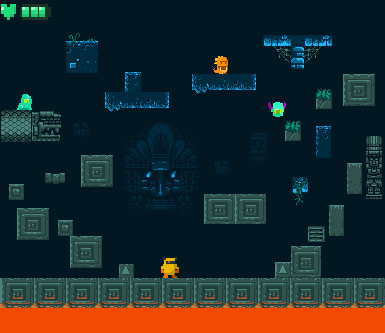
\includegraphics[width=\textwidth, height=15cm]{/home/danhu849/Pictures/game_example.png}}
  \caption{LOFI-exempel Nivå start.\label{fig:4}}
\end{figure}

I övre högra hörnet representeras spelarens återstående liv av gröna kuber i en health-bar. Varje nivå \ref{fig:4} startas med spelkaraktären i nedre delen av spelarfönstret alldeles ovanför lavan.  

\section{Kravformulering}
\subsection{Kravuppfyllelse}
Kraven nedan i \emph{kursivt} är minimikrav som spelet minst måste uppfylla för att godkännas. Nedan specificeras också vilka av våra krav som uppfyller minimikraven.

\subsubsection{\emph{ Spelet ska simulera en 2D-värld i realtid. (Måste vara 2-dimensioner)}}
Uppfylls av ska-krav: 1, 3

\subsubsection{\emph{ Minst 3 typer av objekt. Ska finnas flera instanser av minst två av dessa. Till exempel ett spelarobjekt och många instanser av två olika fiendeobjekt.}}
Uppfylls av ska-krav: 3, 5, 11

\subsubsection{\emph{ Ett beteende som måste finnas med är att figurerna (Objekten) ska röra sig över skärmen. Rörelsen kan följa mönster och/eller vara slumpmässig. Minst ett objekt utöver spelaren ska ha någon typ av rörelse.}}
Uppfylls av ska-krav:5, 11

\subsubsection{\emph{ Ska vara enkelt att modifiera banor i spelet. Det ska vara enkelt att lägga till eller ändra banor i spelet. Detta kan exempelvis lösas genom att läsa in banor från en fil (lite som i Sokoban-labben i TDP002), eller genom att ha funktioner i programkoden som bygger upp en datastruktur som definierar en bana. }}
Uppfylls av ska-krav: 12

\subsubsection{\emph{ Spelet ska upplevas som sammanhängande spel som går att spela.}}
Uppfylls av ska-krav: Alla

\subsubsection{\emph{ En figur ska styras av spelaren, antingen med tangentbordet eller med musen. Du kan även göra ett spel där man spelar två stycken genom att dela på tangentbordet (varje spelare använder olika tangenter). Då styr man var sin figur.}}
Uppfylls av ska-krav: 3

\subsubsection{\emph{ Världen (spelplanen) kan antas vara lika stor som fönstret (du kan göra en större spelplan med scrollning, men det blir lite krångligare).}}
Uppfylls av ska-krav: 1, 4

\subsubsection{\emph{ Det ska finnas kollisionshantering, det vill säga, det ska hända olika saker när objekten möter varandra, de ska påverka varandra på något sätt. T.ex kan ett av objekten tas bort, eller så kan objekten förvandlas på något sätt, eller så kan ett nytt objekt skapas.}}
Uppfylls av ska-krav: 3, 8, 9



\subsection{Ska-krav på projektet}
\begin{enumerate}
\item Spelet ska vara en tvådimensionell platformsscroller där nivån konsekutivt visas desto högre upp spelaren förflyttas.
\item Två spelare ska kunna spela spelet samtidigt. Spelkaraktärerna ha olika färg.
\item Spelet ska ha en startmeny, med möjlighet att ta sig till en nivåmeny, en inställningsmeny genom att klicka på knappar.
\item Spelaren ska kunna röra en spelarfigur i alla vädersträck med piltangenterna och kunna stå och hoppa på plattformar.
\item Spelaren ska efter första hoppet börja bli jagad av stigande lava. Nudas lavan av spelaren ska spelaren dö.
\item Nivån ska avslutas när toppen nås av spelaren eller spelaren avlider.
\item Vid spelarens död ska en Game Over vy visas i spelfönstret.
\item Spelaren ska i luften efter maximal hopphöjd nåtts alltid föras nedåt mot botten av spelskärmen.
\item Projektiler ska kunna avfyras mot den sida spelaren är vänd åt från spelarens position.
\item Projektilerna ska vid kollision med fiender eller väggar upplösas.
\item Spelet ska kunna spelas på skolans datorer.
\item Det ska finnas tre olika typer av fiendeobjekt som har olika utseende. En långsam typ, en flygande typ och en hoppande typ.
\item Nivåer ska kunna läsas in från fil.
\item Det ska finnas en livmätare som visar hur många återstående liv spelaren har.
\item Det ska finnas hp-power-ups som återtillför liv till spelaren vid upplockning om liv saknas.
\item  

\end{enumerate}


\subsection{Bör-krav på projektet}
\begin{enumerate}
\item Spelare ska vid multiplayer kunna välja om "friendly fire" ska vara på eller av i spelets inställningar. 
\item Spelaren ska kunna plocka upp power-ups genom att gå in i samma område som power-up ikonen upptar på spelskärmen. Det finns power-ups som ger spelaren tillbaka liv, möjligheten att hoppa högre samt en power-up som gör att spelaren kan hoppa högre. *
\item Spelet kan spelas med handkontroll. *
\item Animerade sprites (Explosionssprites, rörelse) *
\item Fiender ska kunan avfyra projektiler som färdas i rak bana. *
\item Bosstrid, Vid toppen av berget, under striden med bossen slutar lavan att förflytta sig uppåt och stannar kvar vid spelarfönstrets botten.
\item Spelaren kan få highscore på varje nivå.
\item Ljudeffekter kan spelas upp när spelaren tar skada, avfyrar projektiler och dör. Ljud spelas upp när fiender dör. *
\item Det finns bakgrundsmusik och musik som spelas i nivåerna. *
%\item \subsubsection{Fiendeprojektiler som träffar spelarens projektiler.}
%\subsubsection{Fiendeprojektiler som träffar andra fiendeprojektiler.}
%\subsubsection{Fiendeprojektiler som träffar spelarens projektiler.} 
\end{enumerate}

\subsection{Krav på koden}
\begin{enumerate}
\item    Koden ska följa en accepterad kodstandard. Koden ska gå att kompilera och köra i Ubuntu.
\item    Koden ska vara väldokumenterad. Doxygen ska användas.
\item    "Information hiding" ska användas (ingen åtkomst av instansvariabler utanför klassen).
\item    Designen ska vara modulär med så få beroenden mellan klasser som möjligt.
\item    Det ska finnas en gemensam basklass (Sprite) för alla figurer i programmet. Övriga sprite-figurer ska ärva från denna klass.
\item    Det ska finnas abstrakta metoder, åtminstone för er Sprite-hierarki.
\item    Main-funktionen ska vara liten, huvuddelen av spelet ska finnas i de klasser ni designar. Ett exempel på en lämplig main-funktion:

    int main {
       Game game;
       game.run();
       return 0;
    }
        

\item    Grafiken ska realiseras med hjälp av SFML.
\item    Tillsammans med koden ska en Makefile lämnas in. Handledaren ska kunna köra koden i terminalen med hjälp av denna Makefile.
\end{enumerate}



\end{document}

%%% Local Variables:
%%% mode: latex
%%% TeX-master: t
%%% End:
